\documentclass[1p]{elsarticle_modified}
%\bibliographystyle{elsarticle-num}

%\usepackage[colorlinks]{hyperref}
%\usepackage{abbrmath_seonhwa} %\Abb, \Ascr, \Acal ,\Abf, \Afrak
\usepackage{amsfonts}
\usepackage{amssymb}
\usepackage{amsmath}
\usepackage{amsthm}
\usepackage{scalefnt}
\usepackage{amsbsy}
\usepackage{kotex}
\usepackage{caption}
\usepackage{subfig}
\usepackage{color}
\usepackage{graphicx}
\usepackage{xcolor} %% white, black, red, green, blue, cyan, magenta, yellow
\usepackage{float}
\usepackage{setspace}
\usepackage{hyperref}

\usepackage{tikz}
\usetikzlibrary{arrows}

\usepackage{multirow}
\usepackage{array} % fixed length table
\usepackage{hhline}

%%%%%%%%%%%%%%%%%%%%%
\makeatletter
\renewcommand*\env@matrix[1][\arraystretch]{%
	\edef\arraystretch{#1}%
	\hskip -\arraycolsep
	\let\@ifnextchar\new@ifnextchar
	\array{*\c@MaxMatrixCols c}}
\makeatother %https://tex.stackexchange.com/questions/14071/how-can-i-increase-the-line-spacing-in-a-matrix
%%%%%%%%%%%%%%%

\usepackage[normalem]{ulem}

\newcommand{\msout}[1]{\ifmmode\text{\sout{\ensuremath{#1}}}\else\sout{#1}\fi}
%SOURCE: \msout is \stkout macro in https://tex.stackexchange.com/questions/20609/strikeout-in-math-mode

\newcommand{\cancel}[1]{
	\ifmmode
	{\color{red}\msout{#1}}
	\else
	{\color{red}\sout{#1}}
	\fi
}

\newcommand{\add}[1]{
	{\color{blue}\uwave{#1}}
}

\newcommand{\replace}[2]{
	\ifmmode
	{\color{red}\msout{#1}}{\color{blue}\uwave{#2}}
	\else
	{\color{red}\sout{#1}}{\color{blue}\uwave{#2}}
	\fi
}

\newcommand{\Sol}{\mathcal{S}} %segment
\newcommand{\D}{D} %diagram
\newcommand{\A}{\mathcal{A}} %arc


%%%%%%%%%%%%%%%%%%%%%%%%%%%%%5 test

\def\sl{\operatorname{\textup{SL}}(2,\Cbb)}
\def\psl{\operatorname{\textup{PSL}}(2,\Cbb)}
\def\quan{\mkern 1mu \triangleright \mkern 1mu}

\theoremstyle{definition}
\newtheorem{thm}{Theorem}[section]
\newtheorem{prop}[thm]{Proposition}
\newtheorem{lem}[thm]{Lemma}
\newtheorem{ques}[thm]{Question}
\newtheorem{cor}[thm]{Corollary}
\newtheorem{defn}[thm]{Definition}
\newtheorem{exam}[thm]{Example}
\newtheorem{rmk}[thm]{Remark}
\newtheorem{alg}[thm]{Algorithm}

\newcommand{\I}{\sqrt{-1}}
\begin{document}

%\begin{frontmatter}
%
%\title{Boundary parabolic representations of knots up to 8 crossings}
%
%%% Group authors per affiliation:
%\author{Yunhi Cho} 
%\address{Department of Mathematics, University of Seoul, Seoul, Korea}
%\ead{yhcho@uos.ac.kr}
%
%
%\author{Seonhwa Kim} %\fnref{s_kim}}
%\address{Center for Geometry and Physics, Institute for Basic Science, Pohang, 37673, Korea}
%\ead{ryeona17@ibs.re.kr}
%
%\author{Hyuk Kim}
%\address{Department of Mathematical Sciences, Seoul National University, Seoul 08826, Korea}
%\ead{hyukkim@snu.ac.kr}
%
%\author{Seokbeom Yoon}
%\address{Department of Mathematical Sciences, Seoul National University, Seoul, 08826,  Korea}
%\ead{sbyoon15@snu.ac.kr}
%
%\begin{abstract}
%We find all boundary parabolic representation of knots up to 8 crossings.
%
%\end{abstract}
%\begin{keyword}
%    \MSC[2010] 57M25 
%\end{keyword}
%
%\end{frontmatter}

%\linenumbers
%\tableofcontents
%
\newcommand\colored[1]{\textcolor{white}{\rule[-0.35ex]{0.8em}{1.4ex}}\kern-0.8em\color{red} #1}%
%\newcommand\colored[1]{\textcolor{white}{ #1}\kern-2.17ex	\textcolor{white}{ #1}\kern-1.81ex	\textcolor{white}{ #1}\kern-2.15ex\color{red}#1	}

{\Large $\underline{12a_{0857}~(K12a_{0857})}$}

\setlength{\tabcolsep}{10pt}
\renewcommand{\arraystretch}{1.6}
\vspace{1cm}\begin{tabular}{m{100pt}>{\centering\arraybackslash}m{274pt}}
\multirow{5}{120pt}{
	\centering
	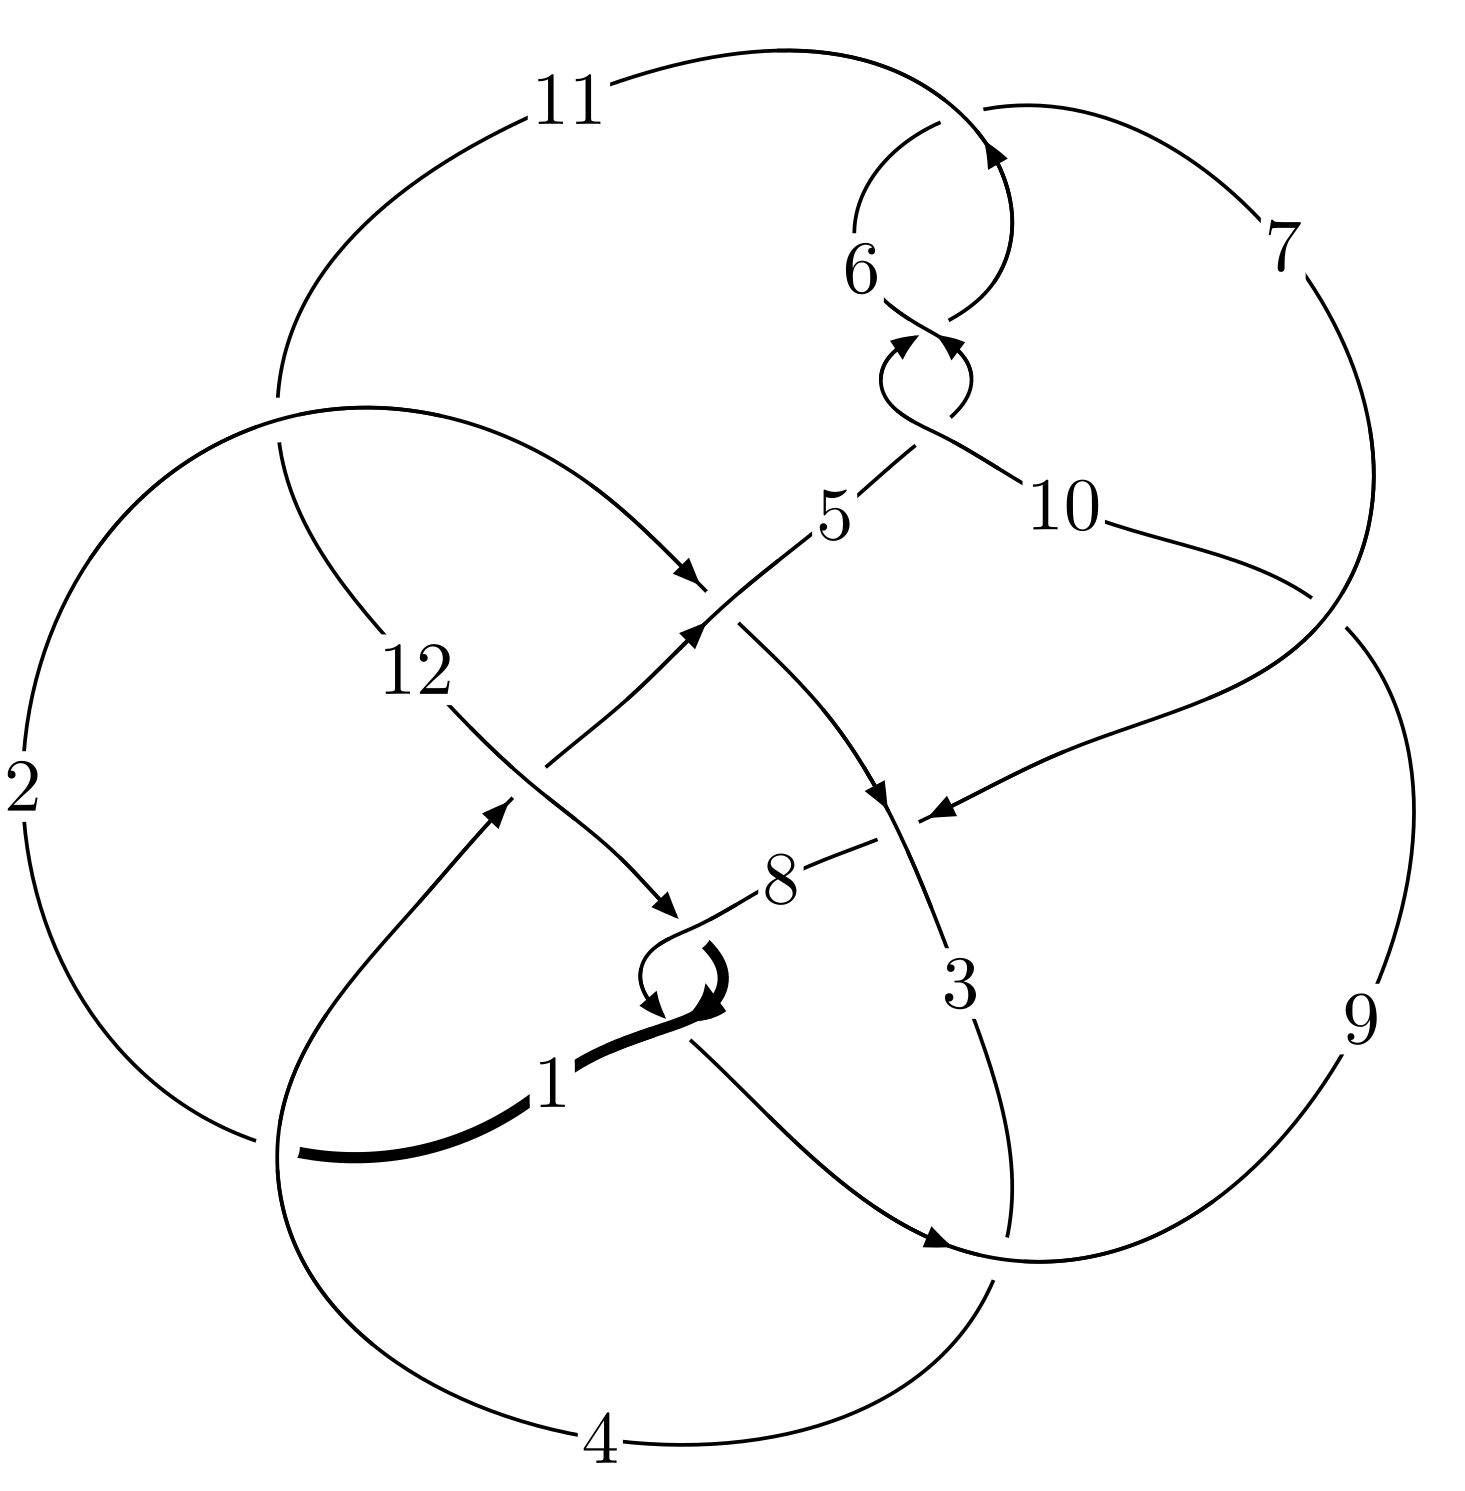
\includegraphics[width=112pt]{../../../GIT/diagram.site/Diagrams/png/1658_12a_0857.png}\\
\ \ \ A knot diagram\footnotemark}&
\allowdisplaybreaks
\textbf{Linearized knot diagam} \\
\cline{2-2}
 &
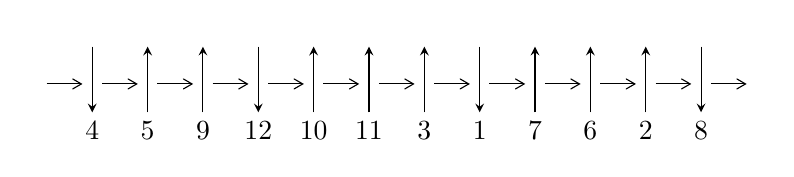
\begin{tikzpicture}[x=20pt, y=17pt]
	% nodes
	\node (C0) at (0, 0) {};
	\node (C1) at (1, 0) {};
	\node (C1U) at (1, +1) {};
	\node (C1D) at (1, -1) {4};

	\node (C2) at (2, 0) {};
	\node (C2U) at (2, +1) {};
	\node (C2D) at (2, -1) {5};

	\node (C3) at (3, 0) {};
	\node (C3U) at (3, +1) {};
	\node (C3D) at (3, -1) {9};

	\node (C4) at (4, 0) {};
	\node (C4U) at (4, +1) {};
	\node (C4D) at (4, -1) {12};

	\node (C5) at (5, 0) {};
	\node (C5U) at (5, +1) {};
	\node (C5D) at (5, -1) {10};

	\node (C6) at (6, 0) {};
	\node (C6U) at (6, +1) {};
	\node (C6D) at (6, -1) {11};

	\node (C7) at (7, 0) {};
	\node (C7U) at (7, +1) {};
	\node (C7D) at (7, -1) {3};

	\node (C8) at (8, 0) {};
	\node (C8U) at (8, +1) {};
	\node (C8D) at (8, -1) {1};

	\node (C9) at (9, 0) {};
	\node (C9U) at (9, +1) {};
	\node (C9D) at (9, -1) {7};

	\node (C10) at (10, 0) {};
	\node (C10U) at (10, +1) {};
	\node (C10D) at (10, -1) {6};

	\node (C11) at (11, 0) {};
	\node (C11U) at (11, +1) {};
	\node (C11D) at (11, -1) {2};

	\node (C12) at (12, 0) {};
	\node (C12U) at (12, +1) {};
	\node (C12D) at (12, -1) {8};
	\node (C13) at (13, 0) {};

	% arrows
	\draw[->,>={angle 60}]
	(C0) edge (C1) (C1) edge (C2) (C2) edge (C3) (C3) edge (C4) (C4) edge (C5) (C5) edge (C6) (C6) edge (C7) (C7) edge (C8) (C8) edge (C9) (C9) edge (C10) (C10) edge (C11) (C11) edge (C12) (C12) edge (C13) ;	\draw[->,>=stealth]
	(C1U) edge (C1D) (C2D) edge (C2U) (C3D) edge (C3U) (C4U) edge (C4D) (C5D) edge (C5U) (C6D) edge (C6U) (C7D) edge (C7U) (C8U) edge (C8D) (C9D) edge (C9U) (C10D) edge (C10U) (C11D) edge (C11U) (C12U) edge (C12D) ;
	\end{tikzpicture} \\
\hhline{~~} \\& 
\textbf{Solving Sequence} \\ \cline{2-2} 
 &
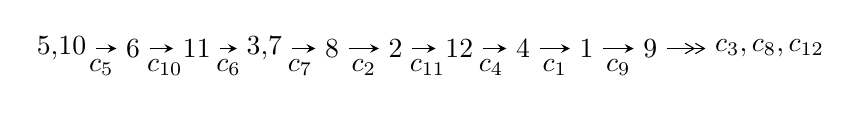
\begin{tikzpicture}[x=23pt, y=7pt]
	% node
	\node (A0) at (-1/8, 0) {5,10};
	\node (A1) at (1, 0) {6};
	\node (A2) at (2, 0) {11};
	\node (A3) at (49/16, 0) {3,7};
	\node (A4) at (33/8, 0) {8};
	\node (A5) at (41/8, 0) {2};
	\node (A6) at (49/8, 0) {12};
	\node (A7) at (57/8, 0) {4};
	\node (A8) at (65/8, 0) {1};
	\node (A9) at (73/8, 0) {9};
	\node (C1) at (1/2, -1) {$c_{5}$};
	\node (C2) at (3/2, -1) {$c_{10}$};
	\node (C3) at (5/2, -1) {$c_{6}$};
	\node (C4) at (29/8, -1) {$c_{7}$};
	\node (C5) at (37/8, -1) {$c_{2}$};
	\node (C6) at (45/8, -1) {$c_{11}$};
	\node (C7) at (53/8, -1) {$c_{4}$};
	\node (C8) at (61/8, -1) {$c_{1}$};
	\node (C9) at (69/8, -1) {$c_{9}$};
	\node (A10) at (11, 0) {$c_{3},c_{8},c_{12}$};

	% edge
	\draw[->,>=stealth]	
	(A0) edge (A1) (A1) edge (A2) (A2) edge (A3) (A3) edge (A4) (A4) edge (A5) (A5) edge (A6) (A6) edge (A7) (A7) edge (A8) (A8) edge (A9) ;
	\draw[->>,>={angle 60}]	
	(A9) edge (A10);
\end{tikzpicture} \\ 

\end{tabular} \\

\footnotetext{
The image of knot diagram is generated by the software ``\textbf{Draw programme}" developed by Andrew Bartholomew(\url{http://www.layer8.co.uk/maths/draw/index.htm\#Running-draw}), where we modified some parts for our purpose(\url{https://github.com/CATsTAILs/LinksPainter}).
}\phantom \\ \newline 
\centering \textbf{Ideals for irreducible components\footnotemark of $X_{\text{par}}$} 
 
\begin{align*}
I^u_{1}&=\langle 
-2.74319\times10^{223} u^{147}+7.21947\times10^{223} u^{146}+\cdots+6.94482\times10^{222} b-1.64886\times10^{223},\\
\phantom{I^u_{1}}&\phantom{= \langle  }-2.55680\times10^{223} u^{147}+1.17756\times10^{224} u^{146}+\cdots+6.94482\times10^{222} a-4.29985\times10^{224},\\
\phantom{I^u_{1}}&\phantom{= \langle  }u^{148}-4 u^{147}+\cdots+28 u+1\rangle \\
I^u_{2}&=\langle 
6 u^{28}+2 u^{27}+\cdots+b-9,\;2 u^{28}-4 u^{27}+\cdots+a+1,\;u^{29}- u^{28}+\cdots+6 u+1\rangle \\
\\
\end{align*}
\raggedright * 2 irreducible components of $\dim_{\mathbb{C}}=0$, with total 177 representations.\\
\footnotetext{All coefficients of polynomials are rational numbers. But the coefficients are sometimes approximated in decimal forms when there is not enough margin.}
\newpage
\renewcommand{\arraystretch}{1}
\centering \section*{I. $I^u_{1}= \langle -2.74\times10^{223} u^{147}+7.22\times10^{223} u^{146}+\cdots+6.94\times10^{222} b-1.65\times10^{223},\;-2.56\times10^{223} u^{147}+1.18\times10^{224} u^{146}+\cdots+6.94\times10^{222} a-4.30\times10^{224},\;u^{148}-4 u^{147}+\cdots+28 u+1 \rangle$}
\flushleft \textbf{(i) Arc colorings}\\
\begin{tabular}{m{7pt} m{180pt} m{7pt} m{180pt} }
\flushright $a_{5}=$&$\begin{pmatrix}1\\0\end{pmatrix}$ \\
\flushright $a_{10}=$&$\begin{pmatrix}0\\u\end{pmatrix}$ \\
\flushright $a_{6}=$&$\begin{pmatrix}1\\- u^2\end{pmatrix}$ \\
\flushright $a_{11}=$&$\begin{pmatrix}u\\- u^3+u\end{pmatrix}$ \\
\flushright $a_{3}=$&$\begin{pmatrix}3.68159 u^{147}-16.9559 u^{146}+\cdots+1057.19 u+61.9145\\3.94998 u^{147}-10.3955 u^{146}+\cdots+26.0103 u+2.37422\end{pmatrix}$ \\
\flushright $a_{7}=$&$\begin{pmatrix}- u^2+1\\u^4-2 u^2\end{pmatrix}$ \\
\flushright $a_{8}=$&$\begin{pmatrix}-2.56776 u^{147}+11.4550 u^{146}+\cdots-390.067 u-4.59737\\-2.17368 u^{147}+6.02080 u^{146}+\cdots+83.1920 u+4.76360\end{pmatrix}$ \\
\flushright $a_{2}=$&$\begin{pmatrix}-0.268390 u^{147}-6.56048 u^{146}+\cdots+1031.18 u+59.5402\\3.94998 u^{147}-10.3955 u^{146}+\cdots+26.0103 u+2.37422\end{pmatrix}$ \\
\flushright $a_{12}=$&$\begin{pmatrix}-4.71414 u^{147}+19.5299 u^{146}+\cdots-986.652 u-49.6532\\1.96876 u^{147}-4.77246 u^{146}+\cdots-106.499 u-3.82153\end{pmatrix}$ \\
\flushright $a_{4}=$&$\begin{pmatrix}3.53479 u^{147}-17.1089 u^{146}+\cdots+1054.78 u+62.0307\\3.40108 u^{147}-8.93411 u^{146}+\cdots+33.4451 u+2.43885\end{pmatrix}$ \\
\flushright $a_{1}=$&$\begin{pmatrix}-7.50495 u^{147}+18.0052 u^{146}+\cdots+157.274 u-8.86158\\-0.207768 u^{147}+1.08489 u^{146}+\cdots-48.3846 u-3.44396\end{pmatrix}$ \\
\flushright $a_{9}=$&$\begin{pmatrix}- u^5+2 u^3- u\\u^7-3 u^5+2 u^3+u\end{pmatrix}$\\&\end{tabular}
\flushleft \textbf{(ii) Obstruction class $= -1$}\\~\\
\flushleft \textbf{(iii) Cusp Shapes $= 23.0139 u^{147}-56.6855 u^{146}+\cdots-967.950 u-41.0456$}\\~\\
\newpage\renewcommand{\arraystretch}{1}
\flushleft \textbf{(iv) u-Polynomials at the component}\newline \\
\begin{tabular}{m{50pt}|m{274pt}}
Crossings & \hspace{64pt}u-Polynomials at each crossing \\
\hline $$\begin{aligned}c_{1}\end{aligned}$$&$\begin{aligned}
&u^{148}+14 u^{147}+\cdots+31659 u+1009
\end{aligned}$\\
\hline $$\begin{aligned}c_{2}\end{aligned}$$&$\begin{aligned}
&u^{148}-3 u^{147}+\cdots-22 u-1
\end{aligned}$\\
\hline $$\begin{aligned}c_{3}\end{aligned}$$&$\begin{aligned}
&u^{148}- u^{147}+\cdots-58242827 u+11140141
\end{aligned}$\\
\hline $$\begin{aligned}c_{4}\end{aligned}$$&$\begin{aligned}
&u^{148}+2 u^{147}+\cdots-56 u+1
\end{aligned}$\\
\hline $$\begin{aligned}c_{5},c_{6},c_{10}\end{aligned}$$&$\begin{aligned}
&u^{148}-4 u^{147}+\cdots+28 u+1
\end{aligned}$\\
\hline $$\begin{aligned}c_{7}\end{aligned}$$&$\begin{aligned}
&u^{148}- u^{147}+\cdots+629 u-841
\end{aligned}$\\
\hline $$\begin{aligned}c_{8},c_{12}\end{aligned}$$&$\begin{aligned}
&u^{148}-2 u^{147}+\cdots-174 u+599
\end{aligned}$\\
\hline $$\begin{aligned}c_{9}\end{aligned}$$&$\begin{aligned}
&u^{148}+12 u^{147}+\cdots+6333548 u+186337
\end{aligned}$\\
\hline $$\begin{aligned}c_{11}\end{aligned}$$&$\begin{aligned}
&u^{148}+15 u^{147}+\cdots+305347 u+14947
\end{aligned}$\\
\hline
\end{tabular}\\~\\
\newpage\renewcommand{\arraystretch}{1}
\flushleft \textbf{(v) Riley Polynomials at the component}\newline \\
\begin{tabular}{m{50pt}|m{274pt}}
Crossings & \hspace{64pt}Riley Polynomials at each crossing \\
\hline $$\begin{aligned}c_{1}\end{aligned}$$&$\begin{aligned}
&y^{148}-34 y^{147}+\cdots-405878435 y+1018081
\end{aligned}$\\
\hline $$\begin{aligned}c_{2}\end{aligned}$$&$\begin{aligned}
&y^{148}+7 y^{147}+\cdots-18 y+1
\end{aligned}$\\
\hline $$\begin{aligned}c_{3}\end{aligned}$$&$\begin{aligned}
&y^{148}+39 y^{147}+\cdots+6412545735582301 y+124102741499881
\end{aligned}$\\
\hline $$\begin{aligned}c_{4}\end{aligned}$$&$\begin{aligned}
&y^{148}-2 y^{147}+\cdots-70 y+1
\end{aligned}$\\
\hline $$\begin{aligned}c_{5},c_{6},c_{10}\end{aligned}$$&$\begin{aligned}
&y^{148}-130 y^{147}+\cdots-174 y+1
\end{aligned}$\\
\hline $$\begin{aligned}c_{7}\end{aligned}$$&$\begin{aligned}
&y^{148}+19 y^{147}+\cdots+90033725 y+707281
\end{aligned}$\\
\hline $$\begin{aligned}c_{8},c_{12}\end{aligned}$$&$\begin{aligned}
&y^{148}-88 y^{147}+\cdots-13930670 y+358801
\end{aligned}$\\
\hline $$\begin{aligned}c_{9}\end{aligned}$$&$\begin{aligned}
&y^{148}+42 y^{147}+\cdots-6491280746914 y+34721477569
\end{aligned}$\\
\hline $$\begin{aligned}c_{11}\end{aligned}$$&$\begin{aligned}
&y^{148}+21 y^{147}+\cdots+9784629847 y+223412809
\end{aligned}$\\
\hline
\end{tabular}\\~\\
\newpage\flushleft \textbf{(vi) Complex Volumes and Cusp Shapes}
$$\begin{array}{c|c|c}  
\text{Solutions to }I^u_{1}& \I (\text{vol} + \sqrt{-1}CS) & \text{Cusp shape}\\
 \hline 
\begin{aligned}
u &= -0.834262 + 0.559566 I \\
a &= -0.128303 + 0.506511 I \\
b &= -0.586616 + 0.645748 I\end{aligned}
 & -2.88757 - 9.19665 I & \phantom{-0.000000 } 0 \\ \hline\begin{aligned}
u &= -0.834262 - 0.559566 I \\
a &= -0.128303 - 0.506511 I \\
b &= -0.586616 - 0.645748 I\end{aligned}
 & -2.88757 + 9.19665 I & \phantom{-0.000000 } 0 \\ \hline\begin{aligned}
u &= -0.882501 + 0.485594 I \\
a &= \phantom{-}0.559978 + 0.598860 I \\
b &= \phantom{-}0.022373 + 0.954432 I\end{aligned}
 & -5.23857 + 1.54918 I & \phantom{-0.000000 } 0 \\ \hline\begin{aligned}
u &= -0.882501 - 0.485594 I \\
a &= \phantom{-}0.559978 - 0.598860 I \\
b &= \phantom{-}0.022373 - 0.954432 I\end{aligned}
 & -5.23857 - 1.54918 I & \phantom{-0.000000 } 0 \\ \hline\begin{aligned}
u &= -0.383892 + 0.898713 I \\
a &= -0.511607 - 0.101872 I \\
b &= -0.265657 - 0.369759 I\end{aligned}
 & -4.40189 + 4.11846 I & \phantom{-0.000000 } 0 \\ \hline\begin{aligned}
u &= -0.383892 - 0.898713 I \\
a &= -0.511607 + 0.101872 I \\
b &= -0.265657 + 0.369759 I\end{aligned}
 & -4.40189 - 4.11846 I & \phantom{-0.000000 } 0 \\ \hline\begin{aligned}
u &= -0.954716 + 0.426398 I \\
a &= -0.328955 - 0.422546 I \\
b &= -0.507598 - 0.928450 I\end{aligned}
 & -5.61580 - 0.33311 I & \phantom{-0.000000 } 0 \\ \hline\begin{aligned}
u &= -0.954716 - 0.426398 I \\
a &= -0.328955 + 0.422546 I \\
b &= -0.507598 + 0.928450 I\end{aligned}
 & -5.61580 + 0.33311 I & \phantom{-0.000000 } 0 \\ \hline\begin{aligned}
u &= \phantom{-}0.828082 + 0.672181 I \\
a &= \phantom{-}0.010750 - 0.276583 I \\
b &= -0.378265 - 0.336048 I\end{aligned}
 & \phantom{-}0.75076 + 2.87734 I & \phantom{-0.000000 } 0 \\ \hline\begin{aligned}
u &= \phantom{-}0.828082 - 0.672181 I \\
a &= \phantom{-}0.010750 + 0.276583 I \\
b &= -0.378265 + 0.336048 I\end{aligned}
 & \phantom{-}0.75076 - 2.87734 I & \phantom{-0.000000 } 0\\
 \hline 
 \end{array}$$\newpage$$\begin{array}{c|c|c}  
\text{Solutions to }I^u_{1}& \I (\text{vol} + \sqrt{-1}CS) & \text{Cusp shape}\\
 \hline 
\begin{aligned}
u &= \phantom{-}0.970690 + 0.468186 I \\
a &= -0.687675 + 0.123557 I \\
b &= -0.877346 + 0.884763 I\end{aligned}
 & -0.01311 - 4.67709 I & \phantom{-0.000000 } 0 \\ \hline\begin{aligned}
u &= \phantom{-}0.970690 - 0.468186 I \\
a &= -0.687675 - 0.123557 I \\
b &= -0.877346 - 0.884763 I\end{aligned}
 & -0.01311 + 4.67709 I & \phantom{-0.000000 } 0 \\ \hline\begin{aligned}
u &= -0.975454 + 0.461950 I \\
a &= -0.919640 - 0.243256 I \\
b &= -0.96455 - 1.05862 I\end{aligned}
 & -3.57878 + 10.72080 I & \phantom{-0.000000 } 0 \\ \hline\begin{aligned}
u &= -0.975454 - 0.461950 I \\
a &= -0.919640 + 0.243256 I \\
b &= -0.96455 + 1.05862 I\end{aligned}
 & -3.57878 - 10.72080 I & \phantom{-0.000000 } 0 \\ \hline\begin{aligned}
u &= \phantom{-}1.096920 + 0.224678 I \\
a &= \phantom{-}1.077810 - 0.355503 I \\
b &= \phantom{-}0.487913 - 0.925485 I\end{aligned}
 & \phantom{-}1.338960 + 0.244377 I & \phantom{-0.000000 } 0 \\ \hline\begin{aligned}
u &= \phantom{-}1.096920 - 0.224678 I \\
a &= \phantom{-}1.077810 + 0.355503 I \\
b &= \phantom{-}0.487913 + 0.925485 I\end{aligned}
 & \phantom{-}1.338960 - 0.244377 I & \phantom{-0.000000 } 0 \\ \hline\begin{aligned}
u &= -0.256354 + 0.830185 I \\
a &= -0.25310 - 1.53553 I \\
b &= \phantom{-}0.283713 - 1.092650 I\end{aligned}
 & -7.23092 - 6.20380 I & \phantom{-0.000000 } 0 \\ \hline\begin{aligned}
u &= -0.256354 - 0.830185 I \\
a &= -0.25310 + 1.53553 I \\
b &= \phantom{-}0.283713 + 1.092650 I\end{aligned}
 & -7.23092 + 6.20380 I & \phantom{-0.000000 } 0 \\ \hline\begin{aligned}
u &= \phantom{-}0.136768 + 0.855356 I \\
a &= \phantom{-}0.706378 + 0.974069 I \\
b &= \phantom{-}0.679992 + 0.579479 I\end{aligned}
 & -2.15264 + 2.82025 I & \phantom{-0.000000 } 0 \\ \hline\begin{aligned}
u &= \phantom{-}0.136768 - 0.855356 I \\
a &= \phantom{-}0.706378 - 0.974069 I \\
b &= \phantom{-}0.679992 - 0.579479 I\end{aligned}
 & -2.15264 - 2.82025 I & \phantom{-0.000000 } 0\\
 \hline 
 \end{array}$$\newpage$$\begin{array}{c|c|c}  
\text{Solutions to }I^u_{1}& \I (\text{vol} + \sqrt{-1}CS) & \text{Cusp shape}\\
 \hline 
\begin{aligned}
u &= -0.217599 + 0.836206 I \\
a &= -0.58507 + 2.16088 I \\
b &= -1.14142 + 1.16900 I\end{aligned}
 & -5.9224 - 15.3515 I & \phantom{-0.000000 } 0 \\ \hline\begin{aligned}
u &= -0.217599 - 0.836206 I \\
a &= -0.58507 - 2.16088 I \\
b &= -1.14142 - 1.16900 I\end{aligned}
 & -5.9224 + 15.3515 I & \phantom{-0.000000 } 0 \\ \hline\begin{aligned}
u &= \phantom{-}0.220795 + 0.835141 I \\
a &= -0.51746 - 1.84375 I \\
b &= -1.08269 - 0.98315 I\end{aligned}
 & -2.33041 + 9.31709 I & \phantom{-0.000000 } 0 \\ \hline\begin{aligned}
u &= \phantom{-}0.220795 - 0.835141 I \\
a &= -0.51746 + 1.84375 I \\
b &= -1.08269 + 0.98315 I\end{aligned}
 & -2.33041 - 9.31709 I & \phantom{-0.000000 } 0 \\ \hline\begin{aligned}
u &= -0.216907 + 0.813285 I \\
a &= \phantom{-}0.03803 + 1.71462 I \\
b &= -0.738737 + 0.926240 I\end{aligned}
 & -7.91109 - 4.12621 I & \phantom{-0.000000 } 0 \\ \hline\begin{aligned}
u &= -0.216907 - 0.813285 I \\
a &= \phantom{-}0.03803 - 1.71462 I \\
b &= -0.738737 - 0.926240 I\end{aligned}
 & -7.91109 + 4.12621 I & \phantom{-0.000000 } 0 \\ \hline\begin{aligned}
u &= -1.137920 + 0.250741 I \\
a &= \phantom{-}1.21331 + 0.81749 I \\
b &= \phantom{-}0.713114 + 1.184890 I\end{aligned}
 & \phantom{-}0.67957 + 2.16426 I & \phantom{-0.000000 } 0 \\ \hline\begin{aligned}
u &= -1.137920 - 0.250741 I \\
a &= \phantom{-}1.21331 - 0.81749 I \\
b &= \phantom{-}0.713114 - 1.184890 I\end{aligned}
 & \phantom{-}0.67957 - 2.16426 I & \phantom{-0.000000 } 0 \\ \hline\begin{aligned}
u &= \phantom{-}0.036176 + 0.778768 I \\
a &= \phantom{-}0.946637 - 0.595588 I \\
b &= -0.038242 - 0.325947 I\end{aligned}
 & -5.69981 + 0.05221 I & \phantom{-0.000000 } 0 \\ \hline\begin{aligned}
u &= \phantom{-}0.036176 - 0.778768 I \\
a &= \phantom{-}0.946637 + 0.595588 I \\
b &= -0.038242 + 0.325947 I\end{aligned}
 & -5.69981 - 0.05221 I & \phantom{-0.000000 } 0\\
 \hline 
 \end{array}$$\newpage$$\begin{array}{c|c|c}  
\text{Solutions to }I^u_{1}& \I (\text{vol} + \sqrt{-1}CS) & \text{Cusp shape}\\
 \hline 
\begin{aligned}
u &= \phantom{-}0.156039 + 0.750413 I \\
a &= \phantom{-}0.97031 + 2.26841 I \\
b &= \phantom{-}1.01555 + 1.09135 I\end{aligned}
 & -1.39682 + 3.46757 I & \phantom{-0.000000 } 0 \\ \hline\begin{aligned}
u &= \phantom{-}0.156039 - 0.750413 I \\
a &= \phantom{-}0.97031 - 2.26841 I \\
b &= \phantom{-}1.01555 - 1.09135 I\end{aligned}
 & -1.39682 - 3.46757 I & \phantom{-0.000000 } 0 \\ \hline\begin{aligned}
u &= -1.232570 + 0.149590 I \\
a &= -1.34678 - 1.81963 I \\
b &= \phantom{-}0.0079557 + 0.0820720 I\end{aligned}
 & -0.65134 + 4.12392 I & \phantom{-0.000000 } 0 \\ \hline\begin{aligned}
u &= -1.232570 - 0.149590 I \\
a &= -1.34678 + 1.81963 I \\
b &= \phantom{-}0.0079557 - 0.0820720 I\end{aligned}
 & -0.65134 - 4.12392 I & \phantom{-0.000000 } 0 \\ \hline\begin{aligned}
u &= -0.130626 + 0.744400 I \\
a &= \phantom{-}0.71695 - 2.90993 I \\
b &= \phantom{-}0.98660 - 1.31247 I\end{aligned}
 & -2.29627 - 5.85849 I & \phantom{-0.000000 } 0 \\ \hline\begin{aligned}
u &= -0.130626 - 0.744400 I \\
a &= \phantom{-}0.71695 + 2.90993 I \\
b &= \phantom{-}0.98660 + 1.31247 I\end{aligned}
 & -2.29627 + 5.85849 I & \phantom{-0.000000 } 0 \\ \hline\begin{aligned}
u &= -0.051336 + 0.751416 I \\
a &= -1.62420 - 0.69229 I \\
b &= -1.46175 - 0.46950 I\end{aligned}
 & -5.98505 + 1.73587 I & \phantom{-0.000000 } 0 \\ \hline\begin{aligned}
u &= -0.051336 - 0.751416 I \\
a &= -1.62420 + 0.69229 I \\
b &= -1.46175 + 0.46950 I\end{aligned}
 & -5.98505 - 1.73587 I & \phantom{-0.000000 } 0 \\ \hline\begin{aligned}
u &= \phantom{-}1.207640 + 0.318226 I \\
a &= \phantom{-}0.531479 + 0.572839 I \\
b &= \phantom{-}0.043236 + 0.652308 I\end{aligned}
 & -2.10884 + 3.92903 I & \phantom{-0.000000 } 0 \\ \hline\begin{aligned}
u &= \phantom{-}1.207640 - 0.318226 I \\
a &= \phantom{-}0.531479 - 0.572839 I \\
b &= \phantom{-}0.043236 - 0.652308 I\end{aligned}
 & -2.10884 - 3.92903 I & \phantom{-0.000000 } 0\\
 \hline 
 \end{array}$$\newpage$$\begin{array}{c|c|c}  
\text{Solutions to }I^u_{1}& \I (\text{vol} + \sqrt{-1}CS) & \text{Cusp shape}\\
 \hline 
\begin{aligned}
u &= -1.216070 + 0.284676 I \\
a &= \phantom{-}0.22126 + 1.44672 I \\
b &= -1.57369 + 0.15677 I\end{aligned}
 & -2.44194 - 5.49792 I & \phantom{-0.000000 } 0 \\ \hline\begin{aligned}
u &= -1.216070 - 0.284676 I \\
a &= \phantom{-}0.22126 - 1.44672 I \\
b &= -1.57369 - 0.15677 I\end{aligned}
 & -2.44194 + 5.49792 I & \phantom{-0.000000 } 0 \\ \hline\begin{aligned}
u &= -1.239860 + 0.173187 I \\
a &= \phantom{-}0.773397 + 0.424869 I \\
b &= \phantom{-}0.68782 + 1.51185 I\end{aligned}
 & \phantom{-}2.37892 + 0.78548 I & \phantom{-0.000000 } 0 \\ \hline\begin{aligned}
u &= -1.239860 - 0.173187 I \\
a &= \phantom{-}0.773397 - 0.424869 I \\
b &= \phantom{-}0.68782 - 1.51185 I\end{aligned}
 & \phantom{-}2.37892 - 0.78548 I & \phantom{-0.000000 } 0 \\ \hline\begin{aligned}
u &= -1.239060 + 0.251944 I \\
a &= \phantom{-}1.43877 + 1.68322 I \\
b &= -1.48406 + 1.39599 I\end{aligned}
 & -2.54709 + 2.50318 I & \phantom{-0.000000 } 0 \\ \hline\begin{aligned}
u &= -1.239060 - 0.251944 I \\
a &= \phantom{-}1.43877 - 1.68322 I \\
b &= -1.48406 - 1.39599 I\end{aligned}
 & -2.54709 - 2.50318 I & \phantom{-0.000000 } 0 \\ \hline\begin{aligned}
u &= \phantom{-}1.262400 + 0.107738 I \\
a &= \phantom{-}1.082500 - 0.540636 I \\
b &= \phantom{-}0.11874 - 1.85691 I\end{aligned}
 & \phantom{-}0.27094 - 4.21563 I & \phantom{-0.000000 } 0 \\ \hline\begin{aligned}
u &= \phantom{-}1.262400 - 0.107738 I \\
a &= \phantom{-}1.082500 + 0.540636 I \\
b &= \phantom{-}0.11874 + 1.85691 I\end{aligned}
 & \phantom{-}0.27094 + 4.21563 I & \phantom{-0.000000 } 0 \\ \hline\begin{aligned}
u &= \phantom{-}1.249400 + 0.260612 I \\
a &= \phantom{-}1.06393 - 1.13172 I \\
b &= -0.997724 - 0.835587 I\end{aligned}
 & \phantom{-}0.53631 + 1.68964 I & \phantom{-0.000000 } 0 \\ \hline\begin{aligned}
u &= \phantom{-}1.249400 - 0.260612 I \\
a &= \phantom{-}1.06393 + 1.13172 I \\
b &= -0.997724 + 0.835587 I\end{aligned}
 & \phantom{-}0.53631 - 1.68964 I & \phantom{-0.000000 } 0\\
 \hline 
 \end{array}$$\newpage$$\begin{array}{c|c|c}  
\text{Solutions to }I^u_{1}& \I (\text{vol} + \sqrt{-1}CS) & \text{Cusp shape}\\
 \hline 
\begin{aligned}
u &= \phantom{-}1.249760 + 0.271941 I \\
a &= \phantom{-}0.35669 - 1.37962 I \\
b &= \phantom{-}0.428838 - 1.124020 I\end{aligned}
 & -2.77756 - 1.61149 I & \phantom{-0.000000 } 0 \\ \hline\begin{aligned}
u &= \phantom{-}1.249760 - 0.271941 I \\
a &= \phantom{-}0.35669 + 1.37962 I \\
b &= \phantom{-}0.428838 + 1.124020 I\end{aligned}
 & -2.77756 + 1.61149 I & \phantom{-0.000000 } 0 \\ \hline\begin{aligned}
u &= \phantom{-}0.243349 + 0.675764 I \\
a &= \phantom{-}0.30508 + 2.50199 I \\
b &= \phantom{-}0.96287 + 1.40677 I\end{aligned}
 & -2.06249 + 6.40773 I & \phantom{-0.000000 } 0. - 10.21181 I \\ \hline\begin{aligned}
u &= \phantom{-}0.243349 - 0.675764 I \\
a &= \phantom{-}0.30508 - 2.50199 I \\
b &= \phantom{-}0.96287 - 1.40677 I\end{aligned}
 & -2.06249 - 6.40773 I & \phantom{-0.000000 -}0. + 10.21181 I \\ \hline\begin{aligned}
u &= \phantom{-}0.027955 + 0.700281 I \\
a &= -0.57906 + 2.74231 I \\
b &= \phantom{-}0.476324 + 0.957322 I\end{aligned}
 & -6.53858 + 5.12910 I & -6.02888 - 5.78970 I \\ \hline\begin{aligned}
u &= \phantom{-}0.027955 - 0.700281 I \\
a &= -0.57906 - 2.74231 I \\
b &= \phantom{-}0.476324 - 0.957322 I\end{aligned}
 & -6.53858 - 5.12910 I & -6.02888 + 5.78970 I \\ \hline\begin{aligned}
u &= \phantom{-}0.582340 + 0.379724 I \\
a &= \phantom{-}1.48013 - 0.01204 I \\
b &= \phantom{-}0.773397 - 0.967716 I\end{aligned}
 & -0.74585 - 2.86716 I & \phantom{-}1.86167 + 3.66817 I \\ \hline\begin{aligned}
u &= \phantom{-}0.582340 - 0.379724 I \\
a &= \phantom{-}1.48013 + 0.01204 I \\
b &= \phantom{-}0.773397 + 0.967716 I\end{aligned}
 & -0.74585 + 2.86716 I & \phantom{-}1.86167 - 3.66817 I \\ \hline\begin{aligned}
u &= \phantom{-}0.029223 + 0.693114 I \\
a &= -0.53721 + 2.04383 I \\
b &= -0.722494 + 1.160630 I\end{aligned}
 & -3.20932 + 1.76134 I & -1.48052 - 3.33045 I \\ \hline\begin{aligned}
u &= \phantom{-}0.029223 - 0.693114 I \\
a &= -0.53721 - 2.04383 I \\
b &= -0.722494 - 1.160630 I\end{aligned}
 & -3.20932 - 1.76134 I & -1.48052 + 3.33045 I\\
 \hline 
 \end{array}$$\newpage$$\begin{array}{c|c|c}  
\text{Solutions to }I^u_{1}& \I (\text{vol} + \sqrt{-1}CS) & \text{Cusp shape}\\
 \hline 
\begin{aligned}
u &= -1.288380 + 0.220568 I \\
a &= -0.310760 + 0.060146 I \\
b &= \phantom{-}1.190800 + 0.741134 I\end{aligned}
 & \phantom{-}2.97962 - 0.43793 I & \phantom{-0.000000 } 0 \\ \hline\begin{aligned}
u &= -1.288380 - 0.220568 I \\
a &= -0.310760 - 0.060146 I \\
b &= \phantom{-}1.190800 - 0.741134 I\end{aligned}
 & \phantom{-}2.97962 + 0.43793 I & \phantom{-0.000000 } 0 \\ \hline\begin{aligned}
u &= -0.055555 + 0.688167 I \\
a &= -1.47974 - 2.87222 I \\
b &= -1.20801 - 1.72162 I\end{aligned}
 & -6.15959 - 5.89642 I & -6.69542 + 6.80189 I \\ \hline\begin{aligned}
u &= -0.055555 - 0.688167 I \\
a &= -1.47974 + 2.87222 I \\
b &= -1.20801 + 1.72162 I\end{aligned}
 & -6.15959 + 5.89642 I & -6.69542 - 6.80189 I \\ \hline\begin{aligned}
u &= \phantom{-}1.302150 + 0.156856 I \\
a &= -0.45371 + 1.69318 I \\
b &= \phantom{-}0.510488 + 0.190093 I\end{aligned}
 & \phantom{-}4.35576 + 0.14805 I & \phantom{-0.000000 } 0 \\ \hline\begin{aligned}
u &= \phantom{-}1.302150 - 0.156856 I \\
a &= -0.45371 - 1.69318 I \\
b &= \phantom{-}0.510488 - 0.190093 I\end{aligned}
 & \phantom{-}4.35576 - 0.14805 I & \phantom{-0.000000 } 0 \\ \hline\begin{aligned}
u &= -1.273880 + 0.332660 I \\
a &= \phantom{-}0.936615 + 0.092078 I \\
b &= -0.1058670 + 0.0205234 I\end{aligned}
 & -1.63408 - 4.06332 I & \phantom{-0.000000 } 0 \\ \hline\begin{aligned}
u &= -1.273880 - 0.332660 I \\
a &= \phantom{-}0.936615 - 0.092078 I \\
b &= -0.1058670 - 0.0205234 I\end{aligned}
 & -1.63408 + 4.06332 I & \phantom{-0.000000 } 0 \\ \hline\begin{aligned}
u &= -1.289870 + 0.273878 I \\
a &= -0.767033 - 0.366375 I \\
b &= -0.55499 - 1.49583 I\end{aligned}
 & \phantom{-}0.89907 - 5.25630 I & \phantom{-0.000000 } 0 \\ \hline\begin{aligned}
u &= -1.289870 - 0.273878 I \\
a &= -0.767033 + 0.366375 I \\
b &= -0.55499 + 1.49583 I\end{aligned}
 & \phantom{-}0.89907 + 5.25630 I & \phantom{-0.000000 } 0\\
 \hline 
 \end{array}$$\newpage$$\begin{array}{c|c|c}  
\text{Solutions to }I^u_{1}& \I (\text{vol} + \sqrt{-1}CS) & \text{Cusp shape}\\
 \hline 
\begin{aligned}
u &= \phantom{-}0.389085 + 0.558326 I \\
a &= \phantom{-}0.618664 - 0.432662 I \\
b &= -0.570599 - 0.187701 I\end{aligned}
 & \phantom{-}1.00696 + 1.85359 I & \phantom{-}7.26628 + 4.55232 I \\ \hline\begin{aligned}
u &= \phantom{-}0.389085 - 0.558326 I \\
a &= \phantom{-}0.618664 + 0.432662 I \\
b &= -0.570599 + 0.187701 I\end{aligned}
 & \phantom{-}1.00696 - 1.85359 I & \phantom{-}7.26628 - 4.55232 I \\ \hline\begin{aligned}
u &= -1.302760 + 0.212861 I \\
a &= -0.29581 - 1.44270 I \\
b &= \phantom{-}0.555211 - 0.959453 I\end{aligned}
 & \phantom{-}3.01507 - 4.85601 I & \phantom{-0.000000 } 0 \\ \hline\begin{aligned}
u &= -1.302760 - 0.212861 I \\
a &= -0.29581 + 1.44270 I \\
b &= \phantom{-}0.555211 + 0.959453 I\end{aligned}
 & \phantom{-}3.01507 + 4.85601 I & \phantom{-0.000000 } 0 \\ \hline\begin{aligned}
u &= -0.176595 + 0.656507 I \\
a &= -0.33129 + 2.39777 I \\
b &= -0.391799 + 0.271433 I\end{aligned}
 & -3.54982 - 6.83567 I & \phantom{-}2.98828 + 11.18078 I \\ \hline\begin{aligned}
u &= -0.176595 - 0.656507 I \\
a &= -0.33129 - 2.39777 I \\
b &= -0.391799 - 0.271433 I\end{aligned}
 & -3.54982 + 6.83567 I & \phantom{-}2.98828 - 11.18078 I \\ \hline\begin{aligned}
u &= -1.290940 + 0.278705 I \\
a &= -1.95472 - 1.34403 I \\
b &= \phantom{-}0.565532 - 0.785691 I\end{aligned}
 & -2.42703 - 8.66471 I & \phantom{-0.000000 } 0 \\ \hline\begin{aligned}
u &= -1.290940 - 0.278705 I \\
a &= -1.95472 + 1.34403 I \\
b &= \phantom{-}0.565532 + 0.785691 I\end{aligned}
 & -2.42703 + 8.66471 I & \phantom{-0.000000 } 0 \\ \hline\begin{aligned}
u &= \phantom{-}1.290760 + 0.320068 I \\
a &= -0.428671 - 0.651956 I \\
b &= -1.37338 + 0.70873 I\end{aligned}
 & -1.80272 + 2.14012 I & \phantom{-0.000000 } 0 \\ \hline\begin{aligned}
u &= \phantom{-}1.290760 - 0.320068 I \\
a &= -0.428671 + 0.651956 I \\
b &= -1.37338 - 0.70873 I\end{aligned}
 & -1.80272 - 2.14012 I & \phantom{-0.000000 } 0\\
 \hline 
 \end{array}$$\newpage$$\begin{array}{c|c|c}  
\text{Solutions to }I^u_{1}& \I (\text{vol} + \sqrt{-1}CS) & \text{Cusp shape}\\
 \hline 
\begin{aligned}
u &= \phantom{-}1.311750 + 0.241225 I \\
a &= -1.24924 + 0.67822 I \\
b &= \phantom{-}1.231930 + 0.218310 I\end{aligned}
 & \phantom{-}3.31278 + 5.59201 I & \phantom{-0.000000 } 0 \\ \hline\begin{aligned}
u &= \phantom{-}1.311750 - 0.241225 I \\
a &= -1.24924 - 0.67822 I \\
b &= \phantom{-}1.231930 - 0.218310 I\end{aligned}
 & \phantom{-}3.31278 - 5.59201 I & \phantom{-0.000000 } 0 \\ \hline\begin{aligned}
u &= \phantom{-}1.307720 + 0.278543 I \\
a &= -1.380210 + 0.080713 I \\
b &= -1.06974 + 2.04051 I\end{aligned}
 & -1.88613 + 9.39814 I & \phantom{-0.000000 } 0 \\ \hline\begin{aligned}
u &= \phantom{-}1.307720 - 0.278543 I \\
a &= -1.380210 - 0.080713 I \\
b &= -1.06974 - 2.04051 I\end{aligned}
 & -1.88613 - 9.39814 I & \phantom{-0.000000 } 0 \\ \hline\begin{aligned}
u &= -0.150051 + 0.630587 I \\
a &= \phantom{-}0.46734 - 2.41428 I \\
b &= \phantom{-}1.10321 - 1.17284 I\end{aligned}
 & -0.81876 - 3.53807 I & \phantom{-}4.00000 + 1.54021 I \\ \hline\begin{aligned}
u &= -0.150051 - 0.630587 I \\
a &= \phantom{-}0.46734 + 2.41428 I \\
b &= \phantom{-}1.10321 + 1.17284 I\end{aligned}
 & -0.81876 + 3.53807 I & \phantom{-}4.00000 - 1.54021 I \\ \hline\begin{aligned}
u &= \phantom{-}1.283320 + 0.450508 I \\
a &= \phantom{-}0.288235 + 0.459970 I \\
b &= \phantom{-}0.607895 - 0.095074 I\end{aligned}
 & \phantom{-}1.26288 + 1.99839 I & \phantom{-0.000000 } 0 \\ \hline\begin{aligned}
u &= \phantom{-}1.283320 - 0.450508 I \\
a &= \phantom{-}0.288235 - 0.459970 I \\
b &= \phantom{-}0.607895 + 0.095074 I\end{aligned}
 & \phantom{-}1.26288 - 1.99839 I & \phantom{-0.000000 } 0 \\ \hline\begin{aligned}
u &= \phantom{-}1.363690 + 0.013125 I \\
a &= -0.868984 + 0.413583 I \\
b &= \phantom{-}1.29272 - 0.70915 I\end{aligned}
 & \phantom{-}6.29495 - 3.07582 I & \phantom{-0.000000 } 0 \\ \hline\begin{aligned}
u &= \phantom{-}1.363690 - 0.013125 I \\
a &= -0.868984 - 0.413583 I \\
b &= \phantom{-}1.29272 + 0.70915 I\end{aligned}
 & \phantom{-}6.29495 + 3.07582 I & \phantom{-0.000000 } 0\\
 \hline 
 \end{array}$$\newpage$$\begin{array}{c|c|c}  
\text{Solutions to }I^u_{1}& \I (\text{vol} + \sqrt{-1}CS) & \text{Cusp shape}\\
 \hline 
\begin{aligned}
u &= \phantom{-}1.36457\phantom{ +0.000000I} \\
a &= \phantom{-}0.800300\phantom{ +0.000000I} \\
b &= -0.265614\phantom{ +0.000000I}\end{aligned}
 & \phantom{-}2.39925\phantom{ +0.000000I} & \phantom{-0.000000 } 0 \\ \hline\begin{aligned}
u &= \phantom{-}0.290323 + 0.556988 I \\
a &= \phantom{-}0.385505 - 1.133770 I \\
b &= -0.323122 - 0.055224 I\end{aligned}
 & \phantom{-}0.85288 + 1.53171 I & \phantom{-}8.92387 - 4.22600 I \\ \hline\begin{aligned}
u &= \phantom{-}0.290323 - 0.556988 I \\
a &= \phantom{-}0.385505 + 1.133770 I \\
b &= -0.323122 + 0.055224 I\end{aligned}
 & \phantom{-}0.85288 - 1.53171 I & \phantom{-}8.92387 + 4.22600 I \\ \hline\begin{aligned}
u &= \phantom{-}1.344750 + 0.313792 I \\
a &= -1.14992 + 1.85647 I \\
b &= \phantom{-}1.16266 + 1.37871 I\end{aligned}
 & \phantom{-}2.35286 + 9.69335 I & \phantom{-0.000000 } 0 \\ \hline\begin{aligned}
u &= \phantom{-}1.344750 - 0.313792 I \\
a &= -1.14992 - 1.85647 I \\
b &= \phantom{-}1.16266 - 1.37871 I\end{aligned}
 & \phantom{-}2.35286 - 9.69335 I & \phantom{-0.000000 } 0 \\ \hline\begin{aligned}
u &= \phantom{-}1.356540 + 0.264667 I \\
a &= -1.17529 + 1.30491 I \\
b &= \phantom{-}1.41228 + 1.12611 I\end{aligned}
 & \phantom{-}3.96376 + 6.83580 I & \phantom{-0.000000 } 0 \\ \hline\begin{aligned}
u &= \phantom{-}1.356540 - 0.264667 I \\
a &= -1.17529 - 1.30491 I \\
b &= \phantom{-}1.41228 - 1.12611 I\end{aligned}
 & \phantom{-}3.96376 - 6.83580 I & \phantom{-0.000000 } 0 \\ \hline\begin{aligned}
u &= \phantom{-}0.616271 + 0.023761 I \\
a &= \phantom{-}0.710288 + 0.110865 I \\
b &= \phantom{-}0.698856 + 0.247047 I\end{aligned}
 & \phantom{-}1.342650 + 0.121848 I & \phantom{-}8.91227 + 0.84671 I \\ \hline\begin{aligned}
u &= \phantom{-}0.616271 - 0.023761 I \\
a &= \phantom{-}0.710288 - 0.110865 I \\
b &= \phantom{-}0.698856 - 0.247047 I\end{aligned}
 & \phantom{-}1.342650 - 0.121848 I & \phantom{-}8.91227 - 0.84671 I \\ \hline\begin{aligned}
u &= \phantom{-}1.363230 + 0.273936 I \\
a &= \phantom{-}0.52798 - 1.81310 I \\
b &= -0.437436 - 0.467247 I\end{aligned}
 & \phantom{-}1.32504 + 10.25150 I & \phantom{-0.000000 } 0\\
 \hline 
 \end{array}$$\newpage$$\begin{array}{c|c|c}  
\text{Solutions to }I^u_{1}& \I (\text{vol} + \sqrt{-1}CS) & \text{Cusp shape}\\
 \hline 
\begin{aligned}
u &= \phantom{-}1.363230 - 0.273936 I \\
a &= \phantom{-}0.52798 + 1.81310 I \\
b &= -0.437436 + 0.467247 I\end{aligned}
 & \phantom{-}1.32504 - 10.25150 I & \phantom{-0.000000 } 0 \\ \hline\begin{aligned}
u &= \phantom{-}1.388500 + 0.091456 I \\
a &= \phantom{-}1.130930 + 0.524621 I \\
b &= -0.840469 + 0.361059 I\end{aligned}
 & \phantom{-}3.75546 - 2.79339 I & \phantom{-0.000000 } 0 \\ \hline\begin{aligned}
u &= \phantom{-}1.388500 - 0.091456 I \\
a &= \phantom{-}1.130930 - 0.524621 I \\
b &= -0.840469 - 0.361059 I\end{aligned}
 & \phantom{-}3.75546 + 2.79339 I & \phantom{-0.000000 } 0 \\ \hline\begin{aligned}
u &= -0.035107 + 0.606267 I \\
a &= \phantom{-}0.184481 - 1.177490 I \\
b &= \phantom{-}1.147090 - 0.469602 I\end{aligned}
 & -0.94271 - 2.50791 I & \phantom{-}2.58911 + 4.37316 I \\ \hline\begin{aligned}
u &= -0.035107 - 0.606267 I \\
a &= \phantom{-}0.184481 + 1.177490 I \\
b &= \phantom{-}1.147090 + 0.469602 I\end{aligned}
 & -0.94271 + 2.50791 I & \phantom{-}2.58911 - 4.37316 I \\ \hline\begin{aligned}
u &= -1.357790 + 0.316689 I \\
a &= -0.71987 - 1.64454 I \\
b &= \phantom{-}1.28709 - 1.16065 I\end{aligned}
 & \phantom{-}3.38172 - 7.33745 I & \phantom{-0.000000 } 0 \\ \hline\begin{aligned}
u &= -1.357790 - 0.316689 I \\
a &= -0.71987 + 1.64454 I \\
b &= \phantom{-}1.28709 + 1.16065 I\end{aligned}
 & \phantom{-}3.38172 + 7.33745 I & \phantom{-0.000000 } 0 \\ \hline\begin{aligned}
u &= -1.404980 + 0.007560 I \\
a &= -0.537581 - 0.104324 I \\
b &= \phantom{-}1.378350 + 0.153884 I\end{aligned}
 & \phantom{-}7.52979 + 0.05295 I & \phantom{-0.000000 } 0 \\ \hline\begin{aligned}
u &= -1.404980 - 0.007560 I \\
a &= -0.537581 + 0.104324 I \\
b &= \phantom{-}1.378350 - 0.153884 I\end{aligned}
 & \phantom{-}7.52979 - 0.05295 I & \phantom{-0.000000 } 0 \\ \hline\begin{aligned}
u &= \phantom{-}1.402850 + 0.118826 I \\
a &= -0.069187 + 0.972484 I \\
b &= \phantom{-}1.212330 - 0.312016 I\end{aligned}
 & \phantom{-}5.92030 + 0.62489 I & \phantom{-0.000000 } 0\\
 \hline 
 \end{array}$$\newpage$$\begin{array}{c|c|c}  
\text{Solutions to }I^u_{1}& \I (\text{vol} + \sqrt{-1}CS) & \text{Cusp shape}\\
 \hline 
\begin{aligned}
u &= \phantom{-}1.402850 - 0.118826 I \\
a &= -0.069187 - 0.972484 I \\
b &= \phantom{-}1.212330 + 0.312016 I\end{aligned}
 & \phantom{-}5.92030 - 0.62489 I & \phantom{-0.000000 } 0 \\ \hline\begin{aligned}
u &= -1.366460 + 0.353854 I \\
a &= -0.362726 - 1.063870 I \\
b &= \phantom{-}0.933679 - 0.734714 I\end{aligned}
 & \phantom{-}2.61058 - 7.13864 I & \phantom{-0.000000 } 0 \\ \hline\begin{aligned}
u &= -1.366460 - 0.353854 I \\
a &= -0.362726 + 1.063870 I \\
b &= \phantom{-}0.933679 + 0.734714 I\end{aligned}
 & \phantom{-}2.61058 + 7.13864 I & \phantom{-0.000000 } 0 \\ \hline\begin{aligned}
u &= -1.39286 + 0.24973 I \\
a &= \phantom{-}0.642759 + 1.045830 I \\
b &= -0.481530 + 0.328023 I\end{aligned}
 & \phantom{-}6.15709 - 4.60004 I & \phantom{-0.000000 } 0 \\ \hline\begin{aligned}
u &= -1.39286 - 0.24973 I \\
a &= \phantom{-}0.642759 - 1.045830 I \\
b &= -0.481530 - 0.328023 I\end{aligned}
 & \phantom{-}6.15709 + 4.60004 I & \phantom{-0.000000 } 0 \\ \hline\begin{aligned}
u &= -1.38851 + 0.28023 I \\
a &= -1.10646 - 1.27908 I \\
b &= \phantom{-}1.25713 - 1.46380 I\end{aligned}
 & \phantom{-}3.10758 - 9.91331 I & \phantom{-0.000000 } 0 \\ \hline\begin{aligned}
u &= -1.38851 - 0.28023 I \\
a &= -1.10646 + 1.27908 I \\
b &= \phantom{-}1.25713 + 1.46380 I\end{aligned}
 & \phantom{-}3.10758 + 9.91331 I & \phantom{-0.000000 } 0 \\ \hline\begin{aligned}
u &= \phantom{-}0.046660 + 0.575990 I \\
a &= \phantom{-}1.39715 + 1.77350 I \\
b &= \phantom{-}0.420585 + 0.622670 I\end{aligned}
 & -1.18014 + 2.00255 I & \phantom{-}1.00660 - 4.20684 I \\ \hline\begin{aligned}
u &= \phantom{-}0.046660 - 0.575990 I \\
a &= \phantom{-}1.39715 - 1.77350 I \\
b &= \phantom{-}0.420585 - 0.622670 I\end{aligned}
 & -1.18014 - 2.00255 I & \phantom{-}1.00660 + 4.20684 I \\ \hline\begin{aligned}
u &= \phantom{-}1.39416 + 0.33770 I \\
a &= \phantom{-}1.03319 - 1.11254 I \\
b &= -0.878878 - 0.875477 I\end{aligned}
 & -2.80416 + 8.28099 I & \phantom{-0.000000 } 0\\
 \hline 
 \end{array}$$\newpage$$\begin{array}{c|c|c}  
\text{Solutions to }I^u_{1}& \I (\text{vol} + \sqrt{-1}CS) & \text{Cusp shape}\\
 \hline 
\begin{aligned}
u &= \phantom{-}1.39416 - 0.33770 I \\
a &= \phantom{-}1.03319 + 1.11254 I \\
b &= -0.878878 + 0.875477 I\end{aligned}
 & -2.80416 - 8.28099 I & \phantom{-0.000000 } 0 \\ \hline\begin{aligned}
u &= \phantom{-}1.39805 + 0.34971 I \\
a &= \phantom{-}0.95239 - 1.52282 I \\
b &= -1.27989 - 1.18958 I\end{aligned}
 & -0.8021 + 19.6275 I & \phantom{-0.000000 } 0 \\ \hline\begin{aligned}
u &= \phantom{-}1.39805 - 0.34971 I \\
a &= \phantom{-}0.95239 + 1.52282 I \\
b &= -1.27989 + 1.18958 I\end{aligned}
 & -0.8021 - 19.6275 I & \phantom{-0.000000 } 0 \\ \hline\begin{aligned}
u &= -1.39897 + 0.34824 I \\
a &= \phantom{-}0.86866 + 1.37304 I \\
b &= -1.23276 + 0.98635 I\end{aligned}
 & \phantom{-}2.80389 - 13.58350 I & \phantom{-0.000000 } 0 \\ \hline\begin{aligned}
u &= -1.39897 - 0.34824 I \\
a &= \phantom{-}0.86866 - 1.37304 I \\
b &= -1.23276 - 0.98635 I\end{aligned}
 & \phantom{-}2.80389 + 13.58350 I & \phantom{-0.000000 } 0 \\ \hline\begin{aligned}
u &= -1.43806 + 0.21229 I \\
a &= \phantom{-}1.161160 + 0.419970 I \\
b &= -0.715032 + 0.140045 I\end{aligned}
 & \phantom{-}6.86268 - 4.69797 I & \phantom{-0.000000 } 0 \\ \hline\begin{aligned}
u &= -1.43806 - 0.21229 I \\
a &= \phantom{-}1.161160 - 0.419970 I \\
b &= -0.715032 - 0.140045 I\end{aligned}
 & \phantom{-}6.86268 + 4.69797 I & \phantom{-0.000000 } 0 \\ \hline\begin{aligned}
u &= \phantom{-}1.41553 + 0.34438 I \\
a &= -0.832851 + 0.755766 I \\
b &= \phantom{-}0.476708 + 1.126080 I\end{aligned}
 & -1.92037 + 10.45010 I & \phantom{-0.000000 } 0 \\ \hline\begin{aligned}
u &= \phantom{-}1.41553 - 0.34438 I \\
a &= -0.832851 - 0.755766 I \\
b &= \phantom{-}0.476708 - 1.126080 I\end{aligned}
 & -1.92037 - 10.45010 I & \phantom{-0.000000 } 0 \\ \hline\begin{aligned}
u &= -1.45751 + 0.09812 I \\
a &= \phantom{-}0.217631 - 0.561349 I \\
b &= \phantom{-}1.085990 + 0.646353 I\end{aligned}
 & \phantom{-}5.76160 + 1.26695 I & \phantom{-0.000000 } 0\\
 \hline 
 \end{array}$$\newpage$$\begin{array}{c|c|c}  
\text{Solutions to }I^u_{1}& \I (\text{vol} + \sqrt{-1}CS) & \text{Cusp shape}\\
 \hline 
\begin{aligned}
u &= -1.45751 - 0.09812 I \\
a &= \phantom{-}0.217631 + 0.561349 I \\
b &= \phantom{-}1.085990 - 0.646353 I\end{aligned}
 & \phantom{-}5.76160 - 1.26695 I & \phantom{-0.000000 } 0 \\ \hline\begin{aligned}
u &= -0.478476 + 0.243406 I \\
a &= \phantom{-}0.716233 - 1.176960 I \\
b &= -0.811165 - 0.122210 I\end{aligned}
 & -1.98595 + 3.98277 I & \phantom{-}5.42042 - 3.64011 I \\ \hline\begin{aligned}
u &= -0.478476 - 0.243406 I \\
a &= \phantom{-}0.716233 + 1.176960 I \\
b &= -0.811165 + 0.122210 I\end{aligned}
 & -1.98595 - 3.98277 I & \phantom{-}5.42042 + 3.64011 I \\ \hline\begin{aligned}
u &= \phantom{-}1.46499 + 0.13521 I \\
a &= \phantom{-}0.446762 - 0.240495 I \\
b &= -0.303105 - 0.313629 I\end{aligned}
 & \phantom{-}2.56788 - 0.11111 I & \phantom{-0.000000 } 0 \\ \hline\begin{aligned}
u &= \phantom{-}1.46499 - 0.13521 I \\
a &= \phantom{-}0.446762 + 0.240495 I \\
b &= -0.303105 + 0.313629 I\end{aligned}
 & \phantom{-}2.56788 + 0.11111 I & \phantom{-0.000000 } 0 \\ \hline\begin{aligned}
u &= -0.360825 + 0.371965 I \\
a &= \phantom{-}1.62925 - 0.96032 I \\
b &= \phantom{-}0.863807 + 0.552007 I\end{aligned}
 & \phantom{-}0.290683 + 1.135740 I & \phantom{-}2.76448 + 3.83447 I \\ \hline\begin{aligned}
u &= -0.360825 - 0.371965 I \\
a &= \phantom{-}1.62925 + 0.96032 I \\
b &= \phantom{-}0.863807 - 0.552007 I\end{aligned}
 & \phantom{-}0.290683 - 1.135740 I & \phantom{-}2.76448 - 3.83447 I \\ \hline\begin{aligned}
u &= -1.48422 + 0.05865 I \\
a &= \phantom{-}0.589184 - 0.135279 I \\
b &= -0.983656 + 0.330263 I\end{aligned}
 & \phantom{-}8.46365 - 4.65317 I & \phantom{-0.000000 } 0 \\ \hline\begin{aligned}
u &= -1.48422 - 0.05865 I \\
a &= \phantom{-}0.589184 + 0.135279 I \\
b &= -0.983656 - 0.330263 I\end{aligned}
 & \phantom{-}8.46365 + 4.65317 I & \phantom{-0.000000 } 0 \\ \hline\begin{aligned}
u &= \phantom{-}1.48915 + 0.05284 I \\
a &= \phantom{-}0.490479 + 0.154722 I \\
b &= -1.091250 - 0.558767 I\end{aligned}
 & \phantom{-}4.85284 + 10.67920 I & \phantom{-0.000000 } 0\\
 \hline 
 \end{array}$$\newpage$$\begin{array}{c|c|c}  
\text{Solutions to }I^u_{1}& \I (\text{vol} + \sqrt{-1}CS) & \text{Cusp shape}\\
 \hline 
\begin{aligned}
u &= \phantom{-}1.48915 - 0.05284 I \\
a &= \phantom{-}0.490479 - 0.154722 I \\
b &= -1.091250 + 0.558767 I\end{aligned}
 & \phantom{-}4.85284 - 10.67920 I & \phantom{-0.000000 } 0 \\ \hline\begin{aligned}
u &= -0.446482 + 0.100884 I \\
a &= -0.003936 - 0.525214 I \\
b &= \phantom{-}0.898860 - 0.773223 I\end{aligned}
 & \phantom{-}0.77460 - 3.01645 I & \phantom{-}6.81557 + 9.13013 I \\ \hline\begin{aligned}
u &= -0.446482 - 0.100884 I \\
a &= -0.003936 + 0.525214 I \\
b &= \phantom{-}0.898860 + 0.773223 I\end{aligned}
 & \phantom{-}0.77460 + 3.01645 I & \phantom{-}6.81557 - 9.13013 I \\ \hline\begin{aligned}
u &= \phantom{-}1.62688\phantom{ +0.000000I} \\
a &= \phantom{-}0.125898\phantom{ +0.000000I} \\
b &= \phantom{-}0.0922858\phantom{ +0.000000I}\end{aligned}
 & \phantom{-}2.90310\phantom{ +0.000000I} & \phantom{-0.000000 } 0 \\ \hline\begin{aligned}
u &= -0.123097 + 0.228309 I \\
a &= \phantom{-}1.96706 - 2.45283 I \\
b &= \phantom{-}0.333029 + 0.484612 I\end{aligned}
 & \phantom{-}0.14087 + 1.58090 I & \phantom{-}1.55742 - 1.87730 I \\ \hline\begin{aligned}
u &= -0.123097 - 0.228309 I \\
a &= \phantom{-}1.96706 + 2.45283 I \\
b &= \phantom{-}0.333029 - 0.484612 I\end{aligned}
 & \phantom{-}0.14087 - 1.58090 I & \phantom{-}1.55742 + 1.87730 I \\ \hline\begin{aligned}
u &= -0.0822211 + 0.0320855 I \\
a &= \phantom{-}4.67861 + 12.51900 I \\
b &= -0.254461 + 1.080010 I\end{aligned}
 & -3.58644 + 4.97395 I & \phantom{-}1.74208 - 5.62080 I \\ \hline\begin{aligned}
u &= -0.0822211 - 0.0320855 I \\
a &= \phantom{-}4.67861 - 12.51900 I \\
b &= -0.254461 - 1.080010 I\end{aligned}
 & -3.58644 - 4.97395 I & \phantom{-}1.74208 + 5.62080 I\\
 \hline 
 \end{array}$$\newpage\newpage\renewcommand{\arraystretch}{1}
\centering \section*{II. $I^u_{2}= \langle 6 u^{28}+2 u^{27}+\cdots+b-9,\;2 u^{28}-4 u^{27}+\cdots+a+1,\;u^{29}- u^{28}+\cdots+6 u+1 \rangle$}
\flushleft \textbf{(i) Arc colorings}\\
\begin{tabular}{m{7pt} m{180pt} m{7pt} m{180pt} }
\flushright $a_{5}=$&$\begin{pmatrix}1\\0\end{pmatrix}$ \\
\flushright $a_{10}=$&$\begin{pmatrix}0\\u\end{pmatrix}$ \\
\flushright $a_{6}=$&$\begin{pmatrix}1\\- u^2\end{pmatrix}$ \\
\flushright $a_{11}=$&$\begin{pmatrix}u\\- u^3+u\end{pmatrix}$ \\
\flushright $a_{3}=$&$\begin{pmatrix}-2 u^{28}+4 u^{27}+\cdots-9 u-1\\-6 u^{28}-2 u^{27}+\cdots+49 u+9\end{pmatrix}$ \\
\flushright $a_{7}=$&$\begin{pmatrix}- u^2+1\\u^4-2 u^2\end{pmatrix}$ \\
\flushright $a_{8}=$&$\begin{pmatrix}12 u^{28}+u^{27}+\cdots-46 u-7\\5 u^{28}+3 u^{27}+\cdots-30 u-6\end{pmatrix}$ \\
\flushright $a_{2}=$&$\begin{pmatrix}4 u^{28}+6 u^{27}+\cdots-58 u-10\\-6 u^{28}-2 u^{27}+\cdots+49 u+9\end{pmatrix}$ \\
\flushright $a_{12}=$&$\begin{pmatrix}2 u^{28}+2 u^{27}+\cdots-24 u-2\\6 u^{28}- u^{27}+\cdots-13 u-1\end{pmatrix}$ \\
\flushright $a_{4}=$&$\begin{pmatrix}- u^{28}+4 u^{27}+\cdots-21 u-3\\-4 u^{28}-2 u^{27}+\cdots+39 u+8\end{pmatrix}$ \\
\flushright $a_{1}=$&$\begin{pmatrix}-12 u^{28}- u^{27}+\cdots+45 u+8\\3 u^{28}-2 u^{27}+\cdots+9 u+3\end{pmatrix}$ \\
\flushright $a_{9}=$&$\begin{pmatrix}- u^5+2 u^3- u\\u^7-3 u^5+2 u^3+u\end{pmatrix}$\\&\end{tabular}
\flushleft \textbf{(ii) Obstruction class $= 1$}\\~\\
\flushleft \textbf{(iii) Cusp Shapes $= 12 u^{28}+u^{27}-177 u^{26}-41 u^{25}+1135 u^{24}+425 u^{23}-4100 u^{22}-2107 u^{21}+8955 u^{20}+5855 u^{19}-11549 u^{18}-9250 u^{17}+7327 u^{16}+7056 u^{15}-241 u^{14}+86 u^{13}-1061 u^{12}-3222 u^{11}-1735 u^{10}-141 u^9+1038 u^8+1862 u^7+1034 u^6-41 u^5-301 u^4-365 u^3-358 u^2-160 u-20$}\\~\\
\newpage\renewcommand{\arraystretch}{1}
\flushleft \textbf{(iv) u-Polynomials at the component}\newline \\
\begin{tabular}{m{50pt}|m{274pt}}
Crossings & \hspace{64pt}u-Polynomials at each crossing \\
\hline $$\begin{aligned}c_{1}\end{aligned}$$&$\begin{aligned}
&u^{29}-15 u^{28}+\cdots+15 u-1
\end{aligned}$\\
\hline $$\begin{aligned}c_{2}\end{aligned}$$&$\begin{aligned}
&u^{29}+14 u^{28}+\cdots+14 u+1
\end{aligned}$\\
\hline $$\begin{aligned}c_{3}\end{aligned}$$&$\begin{aligned}
&u^{29}-2 u^{27}+\cdots+3 u+1
\end{aligned}$\\
\hline $$\begin{aligned}c_{4}\end{aligned}$$&$\begin{aligned}
&u^{29}- u^{28}+\cdots-2 u-1
\end{aligned}$\\
\hline $$\begin{aligned}c_{5},c_{6}\end{aligned}$$&$\begin{aligned}
&u^{29}- u^{28}+\cdots+6 u+1
\end{aligned}$\\
\hline $$\begin{aligned}c_{7}\end{aligned}$$&$\begin{aligned}
&u^{29}+6 u^{27}+\cdots-3 u+1
\end{aligned}$\\
\hline $$\begin{aligned}c_{8}\end{aligned}$$&$\begin{aligned}
&u^{29}+u^{28}+\cdots-2 u+1
\end{aligned}$\\
\hline $$\begin{aligned}c_{9}\end{aligned}$$&$\begin{aligned}
&u^{29}-3 u^{28}+\cdots-10 u+1
\end{aligned}$\\
\hline $$\begin{aligned}c_{10}\end{aligned}$$&$\begin{aligned}
&u^{29}+u^{28}+\cdots+6 u-1
\end{aligned}$\\
\hline $$\begin{aligned}c_{11}\end{aligned}$$&$\begin{aligned}
&u^{29}+2 u^{28}+\cdots+u-1
\end{aligned}$\\
\hline $$\begin{aligned}c_{12}\end{aligned}$$&$\begin{aligned}
&u^{29}- u^{28}+\cdots-2 u-1
\end{aligned}$\\
\hline
\end{tabular}\\~\\
\newpage\renewcommand{\arraystretch}{1}
\flushleft \textbf{(v) Riley Polynomials at the component}\newline \\
\begin{tabular}{m{50pt}|m{274pt}}
Crossings & \hspace{64pt}Riley Polynomials at each crossing \\
\hline $$\begin{aligned}c_{1}\end{aligned}$$&$\begin{aligned}
&y^{29}+7 y^{28}+\cdots-5 y-1
\end{aligned}$\\
\hline $$\begin{aligned}c_{2}\end{aligned}$$&$\begin{aligned}
&y^{29}+8 y^{28}+\cdots+6 y-1
\end{aligned}$\\
\hline $$\begin{aligned}c_{3}\end{aligned}$$&$\begin{aligned}
&y^{29}-4 y^{28}+\cdots-21 y-1
\end{aligned}$\\
\hline $$\begin{aligned}c_{4}\end{aligned}$$&$\begin{aligned}
&y^{29}-5 y^{28}+\cdots+2 y-1
\end{aligned}$\\
\hline $$\begin{aligned}c_{5},c_{6},c_{10}\end{aligned}$$&$\begin{aligned}
&y^{29}-29 y^{28}+\cdots+10 y-1
\end{aligned}$\\
\hline $$\begin{aligned}c_{7}\end{aligned}$$&$\begin{aligned}
&y^{29}+12 y^{28}+\cdots+7 y-1
\end{aligned}$\\
\hline $$\begin{aligned}c_{8},c_{12}\end{aligned}$$&$\begin{aligned}
&y^{29}-15 y^{28}+\cdots+22 y-1
\end{aligned}$\\
\hline $$\begin{aligned}c_{9}\end{aligned}$$&$\begin{aligned}
&y^{29}-5 y^{28}+\cdots+10 y-1
\end{aligned}$\\
\hline $$\begin{aligned}c_{11}\end{aligned}$$&$\begin{aligned}
&y^{29}-2 y^{28}+\cdots+5 y-1
\end{aligned}$\\
\hline
\end{tabular}\\~\\
\newpage\flushleft \textbf{(vi) Complex Volumes and Cusp Shapes}
$$\begin{array}{c|c|c}  
\text{Solutions to }I^u_{2}& \I (\text{vol} + \sqrt{-1}CS) & \text{Cusp shape}\\
 \hline 
\begin{aligned}
u &= -0.999979 + 0.420202 I \\
a &= -0.0487508 + 0.1242170 I \\
b &= \phantom{-}0.122896 - 0.425132 I\end{aligned}
 & \phantom{-}0.90884 - 2.54017 I & \phantom{-}9.49679 + 4.29966 I \\ \hline\begin{aligned}
u &= -0.999979 - 0.420202 I \\
a &= -0.0487508 - 0.1242170 I \\
b &= \phantom{-}0.122896 + 0.425132 I\end{aligned}
 & \phantom{-}0.90884 + 2.54017 I & \phantom{-}9.49679 - 4.29966 I \\ \hline\begin{aligned}
u &= -1.172400 + 0.230229 I \\
a &= \phantom{-}1.221070 + 0.420178 I \\
b &= \phantom{-}0.72438 + 1.39938 I\end{aligned}
 & \phantom{-}1.30589 + 0.94412 I & \phantom{-}3.28599 - 1.78629 I \\ \hline\begin{aligned}
u &= -1.172400 - 0.230229 I \\
a &= \phantom{-}1.221070 - 0.420178 I \\
b &= \phantom{-}0.72438 - 1.39938 I\end{aligned}
 & \phantom{-}1.30589 - 0.94412 I & \phantom{-}3.28599 + 1.78629 I \\ \hline\begin{aligned}
u &= \phantom{-}1.203770 + 0.228092 I \\
a &= \phantom{-}0.161500 - 0.999679 I \\
b &= -0.650867 + 0.762859 I\end{aligned}
 & -1.57852 + 6.79983 I & \phantom{-}3.32887 - 7.87594 I \\ \hline\begin{aligned}
u &= \phantom{-}1.203770 - 0.228092 I \\
a &= \phantom{-}0.161500 + 0.999679 I \\
b &= -0.650867 - 0.762859 I\end{aligned}
 & -1.57852 - 6.79983 I & \phantom{-}3.32887 + 7.87594 I \\ \hline\begin{aligned}
u &= \phantom{-}0.300792 + 0.701944 I \\
a &= -0.272613 - 0.212397 I \\
b &= -0.239857 - 0.472850 I\end{aligned}
 & -4.35092 - 3.59283 I & -0.677700 - 0.091139 I \\ \hline\begin{aligned}
u &= \phantom{-}0.300792 - 0.701944 I \\
a &= -0.272613 + 0.212397 I \\
b &= -0.239857 + 0.472850 I\end{aligned}
 & -4.35092 + 3.59283 I & -0.677700 + 0.091139 I \\ \hline\begin{aligned}
u &= \phantom{-}1.229560 + 0.204644 I \\
a &= \phantom{-}1.42332 - 1.72996 I \\
b &= -0.287250 - 1.327080 I\end{aligned}
 & -1.38475 - 3.11979 I & \phantom{-}2.12057 + 3.22013 I \\ \hline\begin{aligned}
u &= \phantom{-}1.229560 - 0.204644 I \\
a &= \phantom{-}1.42332 + 1.72996 I \\
b &= -0.287250 + 1.327080 I\end{aligned}
 & -1.38475 + 3.11979 I & \phantom{-}2.12057 - 3.22013 I\\
 \hline 
 \end{array}$$\newpage$$\begin{array}{c|c|c}  
\text{Solutions to }I^u_{2}& \I (\text{vol} + \sqrt{-1}CS) & \text{Cusp shape}\\
 \hline 
\begin{aligned}
u &= -0.137523 + 0.716923 I \\
a &= \phantom{-}0.89763 - 2.72112 I \\
b &= \phantom{-}1.12906 - 1.36742 I\end{aligned}
 & -1.71916 - 4.40492 I & -0.59085 + 7.06882 I \\ \hline\begin{aligned}
u &= -0.137523 - 0.716923 I \\
a &= \phantom{-}0.89763 + 2.72112 I \\
b &= \phantom{-}1.12906 + 1.36742 I\end{aligned}
 & -1.71916 + 4.40492 I & -0.59085 - 7.06882 I \\ \hline\begin{aligned}
u &= -1.315220 + 0.042141 I \\
a &= -0.686067 + 0.858758 I \\
b &= \phantom{-}0.876355 + 0.470562 I\end{aligned}
 & \phantom{-}4.00864 + 1.86297 I & \phantom{-}9.44509 - 1.83583 I \\ \hline\begin{aligned}
u &= -1.315220 - 0.042141 I \\
a &= -0.686067 - 0.858758 I \\
b &= \phantom{-}0.876355 - 0.470562 I\end{aligned}
 & \phantom{-}4.00864 - 1.86297 I & \phantom{-}9.44509 + 1.83583 I \\ \hline\begin{aligned}
u &= \phantom{-}0.149040 + 0.644191 I \\
a &= -0.89789 + 2.87024 I \\
b &= \phantom{-}0.033509 + 1.176040 I\end{aligned}
 & -4.63114 + 6.08208 I & -2.19730 - 7.44698 I \\ \hline\begin{aligned}
u &= \phantom{-}0.149040 - 0.644191 I \\
a &= -0.89789 - 2.87024 I \\
b &= \phantom{-}0.033509 - 1.176040 I\end{aligned}
 & -4.63114 - 6.08208 I & -2.19730 + 7.44698 I \\ \hline\begin{aligned}
u &= \phantom{-}1.351680 + 0.301762 I \\
a &= -1.03814 + 1.67297 I \\
b &= \phantom{-}1.38886 + 1.38779 I\end{aligned}
 & \phantom{-}2.98847 + 8.11025 I & \phantom{-}4.16972 - 8.54040 I \\ \hline\begin{aligned}
u &= \phantom{-}1.351680 - 0.301762 I \\
a &= -1.03814 - 1.67297 I \\
b &= \phantom{-}1.38886 - 1.38779 I\end{aligned}
 & \phantom{-}2.98847 - 8.11025 I & \phantom{-}4.16972 + 8.54040 I \\ \hline\begin{aligned}
u &= -1.362600 + 0.278570 I \\
a &= -1.23622 - 1.13259 I \\
b &= \phantom{-}0.319166 - 1.192320 I\end{aligned}
 & \phantom{-}0.18783 - 9.48898 I & \phantom{-}3.31208 + 8.12840 I \\ \hline\begin{aligned}
u &= -1.362600 - 0.278570 I \\
a &= -1.23622 + 1.13259 I \\
b &= \phantom{-}0.319166 + 1.192320 I\end{aligned}
 & \phantom{-}0.18783 + 9.48898 I & \phantom{-}3.31208 - 8.12840 I\\
 \hline 
 \end{array}$$\newpage$$\begin{array}{c|c|c}  
\text{Solutions to }I^u_{2}& \I (\text{vol} + \sqrt{-1}CS) & \text{Cusp shape}\\
 \hline 
\begin{aligned}
u &= -0.477355 + 0.364026 I \\
a &= -0.813650 + 0.175375 I \\
b &= \phantom{-}0.532989 - 0.404192 I\end{aligned}
 & \phantom{-}0.81757 - 2.34791 I & \phantom{-}4.57851 + 8.02025 I \\ \hline\begin{aligned}
u &= -0.477355 - 0.364026 I \\
a &= -0.813650 - 0.175375 I \\
b &= \phantom{-}0.532989 + 0.404192 I\end{aligned}
 & \phantom{-}0.81757 + 2.34791 I & \phantom{-}4.57851 - 8.02025 I \\ \hline\begin{aligned}
u &= \phantom{-}1.410240 + 0.086564 I \\
a &= \phantom{-}0.013047 + 0.669318 I \\
b &= \phantom{-}1.283430 - 0.564993 I\end{aligned}
 & \phantom{-}6.08966 - 0.80590 I & \phantom{-}11.35130 - 0.76639 I \\ \hline\begin{aligned}
u &= \phantom{-}1.410240 - 0.086564 I \\
a &= \phantom{-}0.013047 - 0.669318 I \\
b &= \phantom{-}1.283430 + 0.564993 I\end{aligned}
 & \phantom{-}6.08966 + 0.80590 I & \phantom{-}11.35130 + 0.76639 I \\ \hline\begin{aligned}
u &= \phantom{-}1.44030 + 0.20052 I \\
a &= -1.208130 + 0.321784 I \\
b &= \phantom{-}0.708795 + 0.177396 I\end{aligned}
 & \phantom{-}6.83348 + 4.83072 I & \phantom{-}0.8987 - 31.8055 I \\ \hline\begin{aligned}
u &= \phantom{-}1.44030 - 0.20052 I \\
a &= -1.208130 - 0.321784 I \\
b &= \phantom{-}0.708795 - 0.177396 I\end{aligned}
 & \phantom{-}6.83348 - 4.83072 I & \phantom{-}0.8987 + 31.8055 I \\ \hline\begin{aligned}
u &= -1.65449\phantom{ +0.000000I} \\
a &= -0.0205555\phantom{ +0.000000I} \\
b &= \phantom{-}0.245784\phantom{ +0.000000I}\end{aligned}
 & \phantom{-}2.97055\phantom{ +0.000000I} & \phantom{-}74.7410\phantom{ +0.000000I} \\ \hline\begin{aligned}
u &= -0.293059 + 0.174102 I \\
a &= \phantom{-}1.99518 - 1.27971 I \\
b &= \phantom{-}0.935656 + 0.689805 I\end{aligned}
 & \phantom{-}0.55338 + 1.99406 I & \phantom{-}7.60801 - 2.72974 I \\ \hline\begin{aligned}
u &= -0.293059 - 0.174102 I \\
a &= \phantom{-}1.99518 + 1.27971 I \\
b &= \phantom{-}0.935656 - 0.689805 I\end{aligned}
 & \phantom{-}0.55338 - 1.99406 I & \phantom{-}7.60801 + 2.72974 I\\
 \hline 
 \end{array}$$\newpage
\newpage\renewcommand{\arraystretch}{1}
\centering \section*{ III. u-Polynomials}
\begin{tabular}{m{50pt}|m{274pt}}
Crossings & \hspace{64pt}u-Polynomials at each crossing \\
\hline $$\begin{aligned}c_{1}\end{aligned}$$&$\begin{aligned}
&(u^{29}-15 u^{28}+\cdots+15 u-1)(u^{148}+14 u^{147}+\cdots+31659 u+1009)
\end{aligned}$\\
\hline $$\begin{aligned}c_{2}\end{aligned}$$&$\begin{aligned}
&(u^{29}+14 u^{28}+\cdots+14 u+1)(u^{148}-3 u^{147}+\cdots-22 u-1)
\end{aligned}$\\
\hline $$\begin{aligned}c_{3}\end{aligned}$$&$\begin{aligned}
&(u^{29}-2 u^{27}+\cdots+3 u+1)\\
&\cdot(u^{148}- u^{147}+\cdots-58242827 u+11140141)
\end{aligned}$\\
\hline $$\begin{aligned}c_{4}\end{aligned}$$&$\begin{aligned}
&(u^{29}- u^{28}+\cdots-2 u-1)(u^{148}+2 u^{147}+\cdots-56 u+1)
\end{aligned}$\\
\hline $$\begin{aligned}c_{5},c_{6}\end{aligned}$$&$\begin{aligned}
&(u^{29}- u^{28}+\cdots+6 u+1)(u^{148}-4 u^{147}+\cdots+28 u+1)
\end{aligned}$\\
\hline $$\begin{aligned}c_{7}\end{aligned}$$&$\begin{aligned}
&(u^{29}+6 u^{27}+\cdots-3 u+1)(u^{148}- u^{147}+\cdots+629 u-841)
\end{aligned}$\\
\hline $$\begin{aligned}c_{8}\end{aligned}$$&$\begin{aligned}
&(u^{29}+u^{28}+\cdots-2 u+1)(u^{148}-2 u^{147}+\cdots-174 u+599)
\end{aligned}$\\
\hline $$\begin{aligned}c_{9}\end{aligned}$$&$\begin{aligned}
&(u^{29}-3 u^{28}+\cdots-10 u+1)\\
&\cdot(u^{148}+12 u^{147}+\cdots+6333548 u+186337)
\end{aligned}$\\
\hline $$\begin{aligned}c_{10}\end{aligned}$$&$\begin{aligned}
&(u^{29}+u^{28}+\cdots+6 u-1)(u^{148}-4 u^{147}+\cdots+28 u+1)
\end{aligned}$\\
\hline $$\begin{aligned}c_{11}\end{aligned}$$&$\begin{aligned}
&(u^{29}+2 u^{28}+\cdots+u-1)(u^{148}+15 u^{147}+\cdots+305347 u+14947)
\end{aligned}$\\
\hline $$\begin{aligned}c_{12}\end{aligned}$$&$\begin{aligned}
&(u^{29}- u^{28}+\cdots-2 u-1)(u^{148}-2 u^{147}+\cdots-174 u+599)
\end{aligned}$\\
\hline
\end{tabular}\newpage\renewcommand{\arraystretch}{1}
\centering \section*{ IV. Riley Polynomials}
\begin{tabular}{m{50pt}|m{274pt}}
Crossings & \hspace{64pt}Riley Polynomials at each crossing \\
\hline $$\begin{aligned}c_{1}\end{aligned}$$&$\begin{aligned}
&(y^{29}+7 y^{28}+\cdots-5 y-1)\\
&\cdot(y^{148}-34 y^{147}+\cdots-405878435 y+1018081)
\end{aligned}$\\
\hline $$\begin{aligned}c_{2}\end{aligned}$$&$\begin{aligned}
&(y^{29}+8 y^{28}+\cdots+6 y-1)(y^{148}+7 y^{147}+\cdots-18 y+1)
\end{aligned}$\\
\hline $$\begin{aligned}c_{3}\end{aligned}$$&$\begin{aligned}
&(y^{29}-4 y^{28}+\cdots-21 y-1)\\
&\cdot(y^{148}+39 y^{147}+\cdots+6412545735582301 y+124102741499881)
\end{aligned}$\\
\hline $$\begin{aligned}c_{4}\end{aligned}$$&$\begin{aligned}
&(y^{29}-5 y^{28}+\cdots+2 y-1)(y^{148}-2 y^{147}+\cdots-70 y+1)
\end{aligned}$\\
\hline $$\begin{aligned}c_{5},c_{6},c_{10}\end{aligned}$$&$\begin{aligned}
&(y^{29}-29 y^{28}+\cdots+10 y-1)(y^{148}-130 y^{147}+\cdots-174 y+1)
\end{aligned}$\\
\hline $$\begin{aligned}c_{7}\end{aligned}$$&$\begin{aligned}
&(y^{29}+12 y^{28}+\cdots+7 y-1)\\
&\cdot(y^{148}+19 y^{147}+\cdots+90033725 y+707281)
\end{aligned}$\\
\hline $$\begin{aligned}c_{8},c_{12}\end{aligned}$$&$\begin{aligned}
&(y^{29}-15 y^{28}+\cdots+22 y-1)\\
&\cdot(y^{148}-88 y^{147}+\cdots-13930670 y+358801)
\end{aligned}$\\
\hline $$\begin{aligned}c_{9}\end{aligned}$$&$\begin{aligned}
&(y^{29}-5 y^{28}+\cdots+10 y-1)\\
&\cdot(y^{148}+42 y^{147}+\cdots-6491280746914 y+34721477569)
\end{aligned}$\\
\hline $$\begin{aligned}c_{11}\end{aligned}$$&$\begin{aligned}
&(y^{29}-2 y^{28}+\cdots+5 y-1)\\
&\cdot(y^{148}+21 y^{147}+\cdots+9784629847 y+223412809)
\end{aligned}$\\
\hline
\end{tabular}
\vskip 2pc
\end{document}